\chapter{Perancangan}
\label{chap:perancangan}

Pada bab ini dijelaskan mengenai beberapa perancangan yang dilakukan dalam penelitian ini yaitu rancangan kelas dan rancangan antarmuka pengguna

\section{Rancangan Kelas}
Berdasarkan hasil analisis dari masalah yang dihadapi, dibentuklah diagram kelas pada Gambar \ref{fig:diagramkelas} sebagai gambaran dari perangkat lunak yang akan dibuat.

\begin{figure}[H]
	\begin{center}
		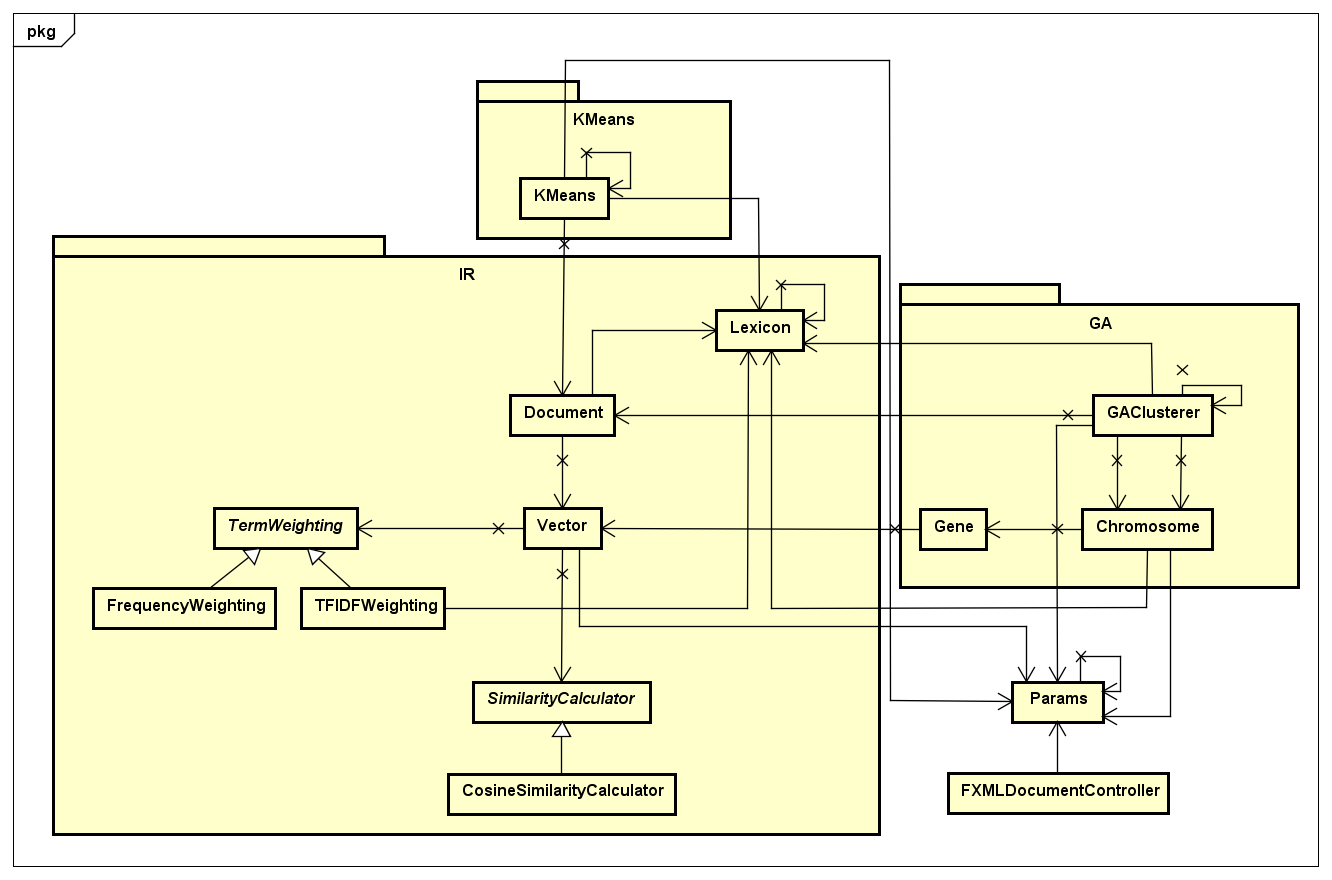
\includegraphics[width=\textwidth]{DiagramKelas/Full}
		\caption{Diagram kelas}
		\label{fig:diagramkelas}
	\end{center}
\end{figure}

Gambar \ref{fig:diagramkelas} merupakan diagram kelas secara umum yang tidak memuat atribut dan \textit{method} dari setiap kelas. Diagram kelas ini sengaja dibuat agar hubungan antar kelas dapat dengan lebih mudah dilihat. Penjelasan dari setiap kelas dalam Gambar \ref{fig:diagramkelas} adalah sebagai berikut.

\subsection{\textit{Document}}

\begin{figure}[H]
	\begin{center}
		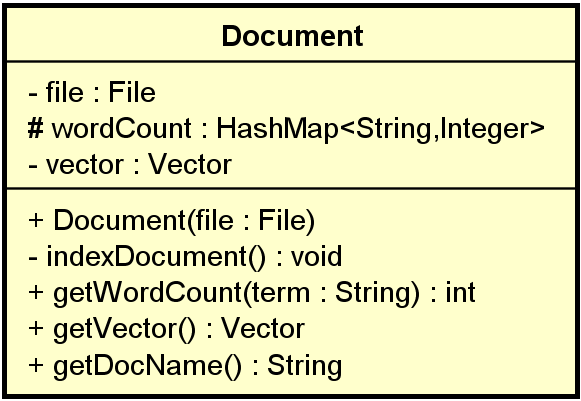
\includegraphics[width=0.4\textwidth]{DiagramKelas/Document}
		\caption{Kelas \textit{Document}}
		\label{fig:kelasDocument}
	\end{center}
\end{figure}

Kelas ini merupakan representasi dari dokumen yang akan diproses dalam pengelompokan. Kelas ini berfungsi untuk menyimpan informasi yang dibutuhkan dari sebuah dokumen selama proses pengelompokan. Atribut yang dimiliki oleh kelas \textit{Document} adalah:

\begin{itemize}
	\item \textit{file}: atribut ini bertipe \textit{File} milik \textit{package} java.io yang berfungsi untuk merepresentasikan \textit{file} dari dokumen yang akan diproses.
	\item \textit{wordCount}: atribut ini bertipe \textit{HashMap} dengan \textit{key} bertipe \textit{String} dan \textit{value} bertipe \textit{Integer}. Atribut ini menyimpan pasangan kata yang dimiliki oleh dokumen tersebut dan frekuensinya.
	\item \textit{vector}: atribut bertipe \textit{Vector} ini merepresentasikan model ruang vektor pada sebuah dokumen.
\end{itemize}

\textit{Method} yang terdapat dalam kelas ini adalah:

\begin{itemize}
	\item \textit{Document}: \textit{method} ini merupakan \textit{constructor} dengan sebuah parameter bertipe \textit{File} yaitu \textit{file} dari dokumen yang akan dikelompokkan.
	\item \textit{indexDocument}: \textit{method} tanpa kembalian (\textit{void}) yang berfungsi untuk mengindeks dokumen untuk mengisi atribut \textit{wordCount}.
	\item \textit{getWordCount}: \textit{method} yang berfungsi untuk mengembalikan banyaknya \textit{term} muncul dalam dokumen.
	\item \textit{getVector}: \textit{method} ini merupakan \textit{getter} dari atribut \textit{vector}.
	\item \textit{getDocName}: \textit{method} ini mengembalikan nama \textit{file} dari dokumen.
\end{itemize}

\subsection{\textit{Vector}}

\begin{figure}[H]
	\begin{center}
		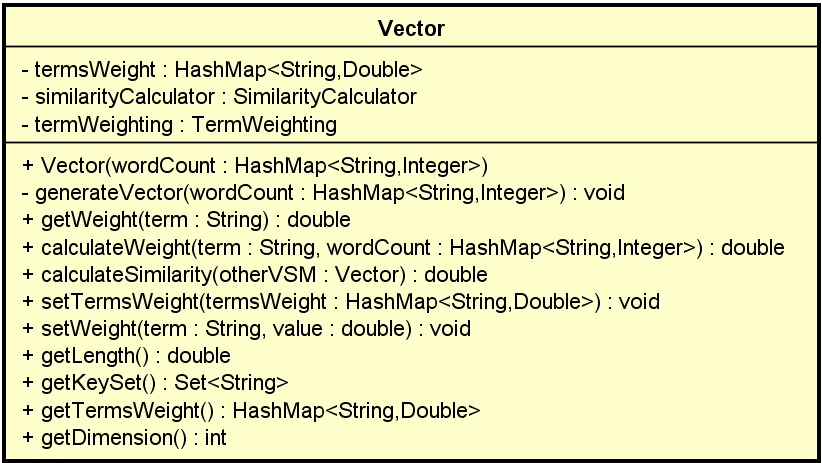
\includegraphics[width=0.7\textwidth]{DiagramKelas/Vector}
		\caption{Kelas \textit{Vector}}
		\label{fig:kelasVector}
	\end{center}
\end{figure}

Kelas ini merupakan kelas yang merepresentasikan sebuah vektor. Kelas ini memiliki fungsi dan atribut yang berfungsi untuk menunjang seluruh aktivitas yang melibatkan suatu vektor. Atribut yang dimiliki kelas ini adalah:

\begin{itemize}
	\item \textit{termsWeight}: atribut ini bertipe \textit{Hashmap} dengan \textit{key} berupa \textit{String} dan \textit{value} berupa \textit{Double}. Atribut ini menyimpan pasangan \term dan bobotnya sesuai dengan metode pembobotan.
	\item \textit{similarityCalculator}: atribut ini bertipe \textit{SimilarityCalculator} dan merupakan objek yang akan digunakan untuk menghitung kemiripan antar vektor.
	\item \textit{termWeighting}: atribut ini bertipe \textit{TermWeighting} dan merupakan objek yang akan digunakan untuk menghitung bobot dari setiap dimensi dalam suatu vektor.
\end{itemize}

\textit{Method} yang terdapat dalam kelas ini adalah:

\begin{itemize}
	\item \textit{Vector}: \textit{method} ini merupakan constructor dengan sebuah parameter yaitu \textit{wordCount} bertipe \textit{Hashmap<String,Integer>} yang merupakan pasangan kata dan banyak kemunculannya dalam dokumen.
	\item \textit{generateVector}: \textit{method} ini merupakan \textit{method} dengan sebuah parameter \textit{Hashmap<String,Integer>} untuk mengisi atribut \textit{termsWeight} dengan bobot tiap \term.
	\item \textit{getWeight}: \textit{method} ini berfungsi untuk mengembalikan bobot dari \term.
	\item \textit{calculateWeight}: \textit{method} ini membutuhkan dua buah parameter yaitu sebuah \term bertipe \textit{String} dan sebuah \textit{Hashmap<String,Integer>}. \textit{Method} ini berfungsi untuk menghitung bobot dari \term berdasarkan frekuensi yang terdapat pada \textit{HashMap}.
	\item \textit{calculateSimilarity}: \textit{method} ini berfungsi untuk menghitung kemiripan (\textit{similarity}) antara vektor ini dengan \textit{otherVector} menggunakan metode yang dipilih oleh pengguna.
	\item \textit{setTermsWeight}: \textit{method} ini merupakan \textit{setter} dari atribut \textit{termsWeight}.
	\item \textit{setWeight}: \textit{method} ini berfungsi untuk mengubah bobot \term menjadi \textit{value}.
	\item \textit{getLength}: \textit{method} ini berfungsi untuk mendapatkan panjang dari vektor.
	\item \textit{getKeyset}: \textit{method} ini berfungsi untuk mendapatkan himpunan \term yang ada pada vektor ini.
	\item \textit{getTermsWeight}: \textit{method} ini merupakan \textit{getter} dari atribut \textit{termsWeight}.
	\item \textit{getDimension}: \textit{method} ini berfungsi untuk mendapatkan besarnya dimensi dari vektor ini.
\end{itemize}

\subsection{\textit{SimilarityCalculator}}

\begin{figure}[H]
	\begin{center}
		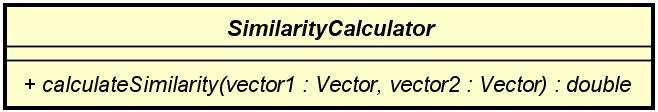
\includegraphics[width=0.6\textwidth]{DiagramKelas/SimilarityCalculator}
		\caption{Kelas \textit{SimilarityCalculator}}
		\label{fig:kelasSimilarityCalculator}
	\end{center}
\end{figure}

Kelas ini merupakan kelas abstrak yang berfungsi untuk menghitung kemiripan antara dua buah objek bertipe \textit{Vector}. Kelas ini tidak memiliki atribut dan hanya memiliki sebuah \textit{method} abstrak yaitu \textit{calculateSimilarity} yang memiliki dua buah parameter \textit{vector1} dan \textit{vector2}. Hasil yang dikembalikan oleh \textit{method} ini adalah kemiripan dari kedua vektor tersebut sesuai dengan metode perhitungan jaraknya.

\subsection{\textit{CosineSimilarityCalculator}}

\begin{figure}[H]
	\begin{center}
		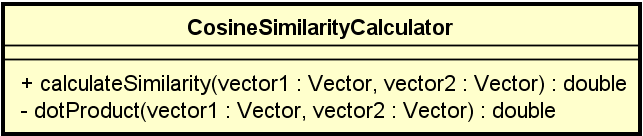
\includegraphics[width=0.6\textwidth]{DiagramKelas/CosineSimilarityCalculator}
		\caption{Kelas \textit{CosineSimilarityCalculator}}
		\label{fig:kelasCosineDist}
	\end{center}
\end{figure}

Kelas ini mengimplementasikan kelas abstrak \textit{SimilarityCalculator}. Kelas ini memiliki satu \textit{method} tambahan selain melakukan \textit{override} pada \textit{method calculateSimilarity}. \textit{Method} yang ada pada kelas ini adalah:

\begin{itemize}
	\item \textit{calculateDistance}: \textit{method} ini merupakan \textit{method} yang diturunkan dari kelas \textit{SimilarityCalculator}. \textit{Method} ini mengembalikan \textit{similarity} dari \textit{vector1} dan \textit{vector2} yang dihitung menggunakan persamaan cosinus (Persamaan \ref{eq:cosine}).
	\item \textit{dotProduct}: \textit{method} ini berfungsi untuk menghitung hasil perkalian titik (\textit{dot product}) antara \textit{vector1} dan \textit{vector2}.
\end{itemize}

\subsection{\textit{TermWeighting}}

\begin{figure}[H]
	\begin{center}
		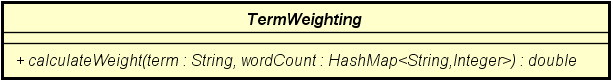
\includegraphics[width=0.6\textwidth]{DiagramKelas/TermWeighting}
		\caption{Kelas \textit{TermWeighting}}
		\label{fig:kelasTermWeighting}
	\end{center}
\end{figure}

Kelas ini merupakan kelas abstrak yang merepresentasikan metode perhitungan bobot dalam suatu vektor. Kelas ini hanya memiliki satu buah \textit{method} yaitu \textit{calculateWeight}. \textit{Method} ini berfungsi untuk menghitung bobot dari \term berdasarkan metode pembobotan yang dipilih oleh pengguna.

\subsection{\textit{FrequencyWeighting}}

\begin{figure}[H]
	\begin{center}
		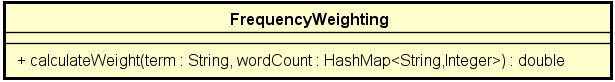
\includegraphics[width=0.6\textwidth]{DiagramKelas/FrequencyWeighting}
		\caption{Kelas \textit{FrequencyWeighting}}
		\label{fig:kelasFrequencyWeighting}
	\end{center}
\end{figure}

Kelas ini mengimplementasikan kelas abstrak \textit{TermWeighting}. Kelas ini hanya memiliki satu \textit{method} yang diturunkan langsung dari kelas \textit{TermWeighting} yaitu \textit{method calculateWeight}. \textit{Method} ini berfungsi untuk menghitung bobot dari \textit{term} menggunakan bobot frekuensi seperti yang telah dijelaskan pada Subbab \ref{sub:freq}.

\subsection{\textit{TFIDFWeighting}}

\begin{figure}[H]
	\begin{center}
		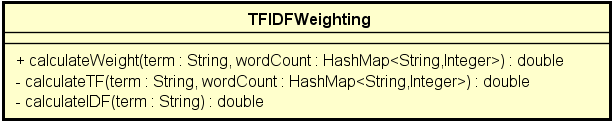
\includegraphics[width=0.6\textwidth]{DiagramKelas/TFIDFWeighting}
		\caption{Kelas \textit{TFIDFWeighting}}
		\label{fig:kelasTFIDFWeighting}
	\end{center}
\end{figure}

Kelas ini mengimplementasikan kelas abstrak \textit{TermWeighting}. Kelas ini memiliki dua \textit{method} tambahan selain melakukan \textit{override} pada \textit{method calculateWeight}. \textit{Method} yang ada pada kelas ini adalah:

\begin{itemize}
	\item \textit{calculateWeight}: \textit{method} ini merupakan \textit{method} yang diturunkan dari kelas \textit{TermWeighting}. \textit{Method} ini mengembalikan bobot dari \term yang dihitung menggunakan teknik TF-IDF.
	\item \textit{calculateTF}: \textit{method} ini berfungsi untuk menghitung \textit{TF} dari suatu \textit{term}.
	\item \textit{calculateIDF}: \textit{method} ini berfungsi untuk menghitung \textit{IDF} dari suatu \textit{term}.
\end{itemize}

\subsection{\textit{Lexicon}}

\begin{figure}[H]
	\begin{center}
		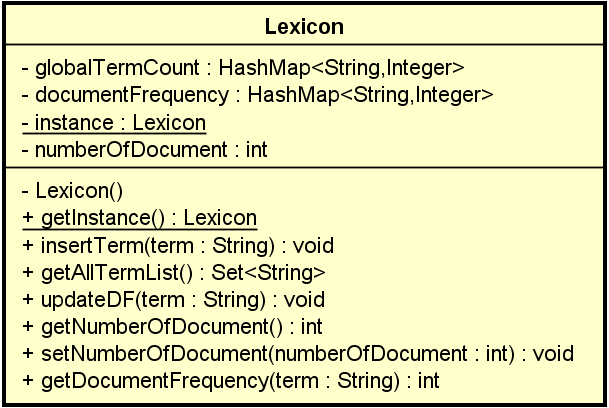
\includegraphics[width=0.55\textwidth]{DiagramKelas/Lexicon}
		\caption{Kelas \textit{Lexicon}}
		\label{fig:kelasLexicon}
	\end{center}
\end{figure}

Kelas ini merepresentasikan sebuah kamus yang menangani seluruh kebutuhan dalam proses pengelompokan yang membutuhkan akses global untuk keseluruhan koleksi dokumen. Atribut yang ada dalam kelas ini adalah:

\begin{itemize}
	\item \textit{globalTermCount}: atribut ini bertipe \textit{HashMap} dengan \textit{key} bertipe \textit{String} dan \textit{value} bertipe \textit{Integer}. Atribut ini berfungsi untuk menyimpan seluruh \term yang muncul dan banyak kemunculannya dalam keseluruhan koleksi dokumen.
	\item \textit{documentFrequency}: atribut ini bertipe \textit{HashMap} dengan \textit{key} bertipe \textit{String} dan \textit{value} bertipe \textit{Integer}. Atribut ini berfungsi untuk menyimpan seluruh frekuensi dokumen dari tiap term.
	\item \textit{instance}: atribut ini merupakan objek bertipe \textit{Lexicon} sebagai instansiasi satu-satunya dari kelas \textit{Lexicon} karena kelas ini bersifat \textit{singleton}.
	\item \textit{numberOfDocument}: atribut ini menyimpan banyaknya dokumen yang terdaftar di \textit{Lexicon}. 
\end{itemize}

\textit{Method} yang ada pada kelas ini adalah:

\begin{itemize}
	\item \textit{Lexicon}: \textit{method} ini merupakan \textit{constructor private} untuk menjamin tidak akan ada lebih dari satu \textit{instance} selama perangkat lunak berjalan.
	\item \textit{getInstance}: \textit{method} ini merupakan \textit{method static} yang berfungsi sebagai \textit{getter} dari atribut \textit{instance}.
	\item \textit{insertTerm}: \textit{method} ini berfungsi untuk memasukkan \textit{term} ke dalam atribut \textit{globalTermCount}.
	\item \textit{getAllTermList}: \textit{method} ini bertugas mengembalikan daftar seluruh \term yang pernah muncul di seluruh koleksi dokumen.
	\item \textit{updateDF}: \textit{method} ini berfungsi untuk menambah nilai TF dari \term "\textit{term}".
	\item \textit{getNumberOfDocument}: \textit{method} ini merupakan \textit{getter} dari atribut \textit{numberOfDocument}.
	\item \textit{setNumberOfDocument}: \textit{method} ini merupakan \textit{setter} dari atribut \textit{numberOfDocument}.
	\item \textit{getDocumentFrequency}: \textit{method} ini berfungsi untuk mendapatkan nilai DF dari \term "\textit{term}".
\end{itemize}

\subsection{\textit{Gene}}

\begin{figure}[H]
	\begin{center}
		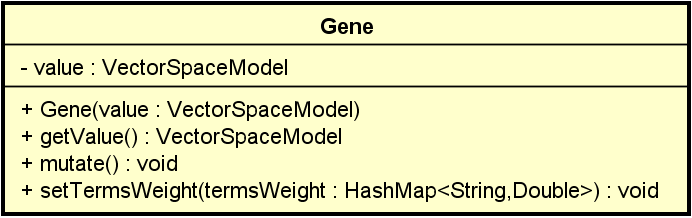
\includegraphics[width=0.25\textwidth]{DiagramKelas/Gene}
		\caption{Kelas \textit{Gene}}
		\label{fig:kelasGene}
	\end{center}
\end{figure}

Kelas ini merepresentasikan gen dalam algoritma genetika. Kelas ini hanya memiliki sebuah atribut \textit{value} bertipe \textit{Vector}. Atribut ini menyimpan vektor yang menjadi titik pusat \textit{cluster} (\textit{centroid}). \textit{Method} yang ada pada kelas ini adalah:

\begin{itemize}
	\item \textit{Gene}: \textit{method} ini merupakan \textit{constructor} dari kelas \textit{Gene} yang membutuhkan sebuah parameter bertipe \textit{Vector} untuk mengisi atribut \textit{value}.
	\item \textit{getValue}: \textit{method} ini merupakan \textit{getter} dari atribut \textit{value}.
	\item \textit{mutate}: \textit{method} ini berfungsi untuk melakukan mutasi pada gen. \textit{Method} ini sebenarnya hanya bertugas memanggil fungsi \textit{mutate()} dari atribut \textit{value}.
\end{itemize}

\subsection{\textit{Chromosome}}

\begin{figure}[H]
	\begin{center}
		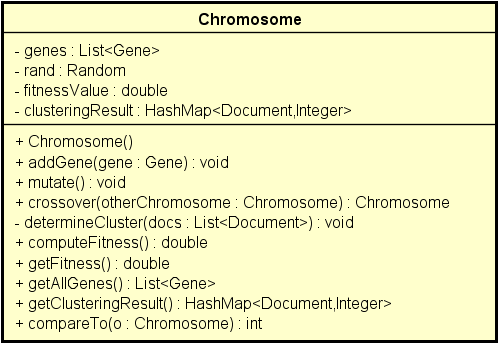
\includegraphics[width=0.6\textwidth]{DiagramKelas/Chromosome}
		\caption{Kelas \textit{Chromosome}}
		\label{fig:kelasChromosome}
	\end{center}
\end{figure}

Kelas ini merepresentasikan kromosom dalam algoritma genetika (Subbab \ref{sub:chromosome}). Atribut yang terdapat dalam kelas ini adalah:

\begin{itemize}
	\item \textit{genes}: atribut bertipe \textit{List of Gene} dan merupakan kumpulan gen yang terdapat dalam kromosom.
	\item \textit{rand}: atribut ini merupakan objek \textit{Random} milik \textit{Java} dan berfungsi untuk membangkitkan bilangan acak yang dibutuhkan dalam setiap proses dalam kromosom.
	\item \textit{fitnessValue}: atribut ini menyimpan nilai \textit{fitness} dari kromosom.
	\item \textit{clusteringResult}: atribut ini akan menyimpan hasil dari pengelompokan. Atribut ini bertipe \textit{HashMap} yang menyimpan pasangan dokumen dan \textit{cluster} dari dokumen tersebut.
\end{itemize}

\textit{Method} yang terdapat dalam kelas ini adalah:

\begin{itemize}
	\item \textit{Chromosome}: \textit{method} ini merupakan \textit{constructor} tanpa parameter untuk membentuk objek dari kelas \textit{Chromosome}.
	\item \textit{addGene}: \textit{method} ini bertugas untuk menambahkan satu gen ke dalam kromosom (ke dalam atribut \textit{genes}).
	\item \textit{mutate}: \textit{method} ini berfungsi untuk melakukan mutasi pada kromosom dengan cara melakukan mutasi pada sebuah gen secara acak (Subbab \ref{sub:mutation}).
	\item \textit{crossover}: \textit{method} ini bertugas untuk melakukan persilangan dengan kromosom \textit{otherChromosome} untuk mengahsilkan keturunan (Subbab \ref{sub:crossover}).
	\item \textit{determineCluster}: \textit{method} ini berfungsi untuk menentukan keanggotaan dari setiap dokumen.
	\item \textit{computeFitness}: \textit{method} ini mengembalikan nilai \textit{fitness} dari kromosom (Subbab \ref{sub:fitnessFn}).
	\item \textit{getFitness}: \textit{method} ini merupakan \textit{getter} dari atribut \textit{fitnessValue}.
	\item \textit{getAllGenes}: \textit{method} ini merupakan \textit{getter} dari atribut \textit{genes}.
	\item \textit{getClusteringResult}: \textit{method} ini merupakan \textit{getter} dari atribut \textit{clusteringResult}.
	\item \textit{compareTo}: \textit{method} ini merupakan turunan dari \textit{interface Comparable} milik \textit{Java} yang dibutuhkan untuk membandingkan kromosom ini dengan kromosom \textit{o}. Method ini nantinya akan digunakan dalam proses \textit{sorting}.
\end{itemize}

\subsection{\textit{GAClusterer}}

\begin{figure}[H]
	\begin{center}
		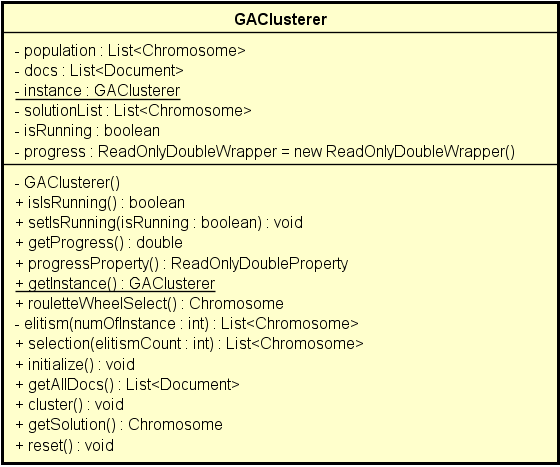
\includegraphics[width=0.7\textwidth]{DiagramKelas/GAClusterer}
		\caption{Kelas \textit{GAClusterer}}
		\label{fig:kelasGAClusterer}
	\end{center}
\end{figure}

Kelas ini merupakan kelas utama yang akan mengatur jalannya proses pengelompokan menggunakan algoritma genetika. Kelas ini merupakan kelas \textit{singleton}. Atribut yang terdapat dalam kelas ini adalah:

\begin{itemize}
	\item \textit{population}: atribut ini bertipe \textit{List of Chromosome} yang merepresentasikan populasi pada generasi saat ini.
	\item \textit{docs}: atribut ini bertipe \textit{List of Document} yang berfungsi untuk menyimpan seluruh koleksi dokumen.
	\item \textit{instance}: atribut \textit{static} ini berfungsi untuk menyimpan \textit{instance} dari kelas \textit{GAClusterer}.
	\item \textit{solutionList}: atribut ini bertipe \textit{List of Chromosome} yang mencatat kromosom dengan nilai \textit{fitness} terbaik untuk setiap generasinya.
	\item \textit{isRunning}: atribut ini berfungsi untuk menyimpan status dari operasi pengelompokan menggunakan GA. Apabila bernilai \textit{true} maka program sedang berjalan dan \textit{false} apabila tidak sedang berjalan.
	\item \textit{progress}: atribut ini bertipe \textit{ReadOnlyDoubleWrapper} dan berfungsi untuk menyimpan perkembangan dari pengerjaan tugas pengelompokan ini ke antarmuka pengguna.
\end{itemize}

\textit{Method} yang terdapat dalam kelas ini adalah:

\begin{itemize}
	\item \textit{GAClusterer}: \textit{method} ini merupakan \textit{constructor private} yang berfungsi untuk menjamin tidak akan ada \textit{instance} dibuat diluar dari kelas ini.
	\item \textit{setIsRunning}: \textit{method} ini mrupakan \textit{setter} dari atribut \textit{isRunning}.
	\item \textit{getProgress}: \textit{method} ini mengembalikan perkembangan pekerjaan program (skala 0 sampai dengan 1).
	\item \textit{progressProperty}: \textit{method} ini merupakan \textit{getter} dari atribut \textit{progress}.
	\item \textit{getInstance}: \textit{method} ini merupakan \textit{getter} dari atribut \textit{instance}.
	\item \textit{rouletteWheelSelect}: \textit{method} ini bertugas untuk memilih sebuah kromosom menggunakan teknik \textit{roulette-wheel selection} dari populasi.
	\item \textit{elitism}: \textit{method} ini bertugas untuk memilih $n$ kromosom elit yang akan langsung masuk ke generasi berikutnya.
	\item \textit{selection}: \textit{method} ini bertugas untuk melakukan \textit{roulette-wheel selection} sebanyak populasi untuk menghasilkan populasi dari generasi selanjutnya.
	\item \textit{initialize}: \textit{method} ini berfungsi untuk melakukan \textit{indexing} dokumen dan membentuk populasi awal.
	\item \textit{getAllDocs}: \textit{method} ini merupakan \textit{getter} dari atribut \textit{docs}.
	\item \textit{cluster}: \textit{method} ini merupakan \textit{method} utama yang bertugas melakukan pengelompokan dokumen dengan menggunakan algoritma genetika.
	\item \textit{getSolution}: \textit{method} ini berfungsi untuk menggembalikan solusi dari proses pengelompokan menggunakan algoritma genetika.
	\item \textit{reset}: \textit{method} ini berfungsi untuk mengatur ulang seluruh atribut untuk proses pengelompokan berikutnya.
\end{itemize}

\subsection{\textit{Params}}

\begin{figure}[H]
	\begin{center}
		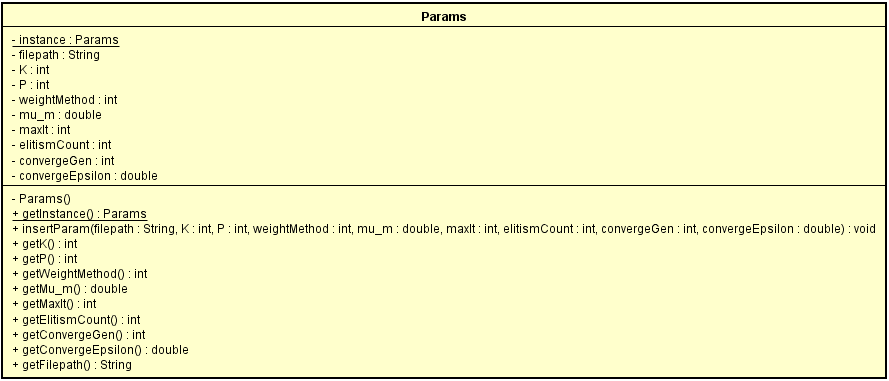
\includegraphics[width=\textwidth]{DiagramKelas/Params}
		\caption{Kelas \textit{Params}}
		\label{fig:kelasParams}
	\end{center}
\end{figure}

Kelas ini berfungsi untuk menyimpan seluruh parameter yang diberikan oleh pengguna agar dapat digunakan oleh setiap kelas yang membutuhkannya. Kelas ini bersifat \textit{singleton} sehingga hanya akan ada satu buah \textit{instance} selama perangkat lunak berjalan. Atribut yang ada dalam kelas ini adalah:

\begin{itemize}
	\item \textit{instance}: atribut ini merupakan objek bertipe \textit{Params} sebagai instansiasi satu-satunya dari kelas \textit{Params} karena kelas ini bersifat \textit{singleton}.
	\item \textit{filepath}: atribut ini berfungsi untuk menyimpan alamat dari direktori dokumen yang akan dikelompokkan.
	\item \textit{K}: atribut ini berfungsi untuk menyimpan banyaknya \textit{cluster} yang akan dipentuk dalam proses pengelompokan.
	\item \textit{P}: atribut ini berfungsi untuk menyimpan banyaknya populasi yang akan dibentuk dalam proses pengelompokan menggunakan algoritma genetika.
	\item \textit{weightingMethod}: atribut ini berfungsi untuk menyimpan metode pembobotan yang akan digunakan dalam proses pengelompokan. Apabila atribut ini bernilai 0 maka metode yang digunakan adalah TF-IDF sedangkan apabila bernilai 1 maka metode yang akan digunakan adalah bobot frekuensi.
	\item \textit{mu}\_\textit{m}: atribut ini berfungsi untuk menyimpan probabilitas mutasi dalam bentuk bilangan riil bernilai antara 0 sampai dengan 1.
	\item \textit{maxIt}: atribut ini berfungsi untuk menyimpan banyaknya iterasi maksimal yang dapat dilakukan.
	\item \textit{elitismCount}: atribut ini berfungsi untuk menyimpan banyaknya individu yang akan dijadikan elit pada tahap seleksi.
	\item \textit{convergeGen}: atribut ini berfungsi untuk menyimpan banyaknya generasi konvergen sebelum proses pengelompokan diberhentikan.
	\item \textit{convergeEpsilon}: atribut ini berfungsi untuk menyimpan nilai yang akan digunakan untuk membandingkan \textit{fitness} tiap solusi dari setiap generasi untuk menentukan apakah sudah tercapai konvergen atau belum.
\end{itemize}

\textit{Method} yang ada pada kelas ini adalah:

\begin{itemize}
	\item \textit{Params}: \textit{method} ini merupakan \textit{constructor private} untuk menjamin tidak akan ada lebih dari satu \textit{instance} selama perangkat lunak berjalan.
	\item \textit{getInstance}: \textit{method} ini merupakan \textit{method static} yang berfungsi sebagai \textit{getter} dari atribut \textit{instance}.
	\item \textit{insertParam}: \textit{method} ini bertugas untuk memasukkan atau mengubah nilai dari setiap atribut dalam kelas ini.
	\item \textit{getK}: \textit{method} ini merupakan \textit{getter} dari atribut \textit{K}.
	\item \textit{getP}: \textit{method} ini merupakan \textit{getter} dari atribut \textit{P}.
	\item \textit{getWeightingMethod}: \textit{method} ini merupakan \textit{getter} dari atribut \textit{weightingMethod}.
	\item \textit{getMu}\_\textit{m}: \textit{method} ini merupakan \textit{getter} dari atribut \textit{mu}\_\textit{m}.
	\item \textit{getMaxIt}: \textit{method} ini merupakan \textit{getter} dari atribut \textit{maxIt}.
	\item \textit{getElitismCount}: \textit{method} ini merupakan \textit{getter} dari atribut \textit{elitismCount}.
	\item \textit{getConvergeGen}: \textit{method} ini merupakan \textit{getter} dari atribut \textit{convergeGen}.
	\item \textit{getConvergeEpsilon}: \textit{method} ini merupakan \textit{getter} dari atribut \textit{convergeEpsilon}.
	\item \textit{getFilepath}: \textit{method} ini merupakan \textit{getter} dari atribut \textit{filepath}.
\end{itemize}.

\subsection{\textit{KMeans}}

\begin{figure}[H]
	\begin{center}
		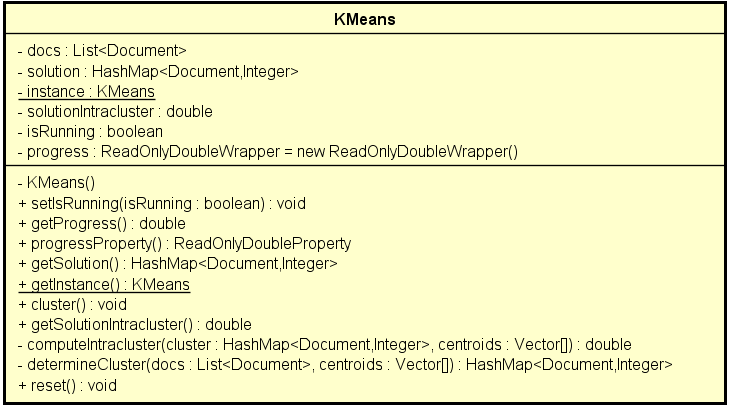
\includegraphics[width=0.75\textwidth]{DiagramKelas/KMeans}
		\caption{Kelas \textit{KMeans}}
		\label{fig:kelasKMeans}
	\end{center}
\end{figure}

Kelas ini merupakan kelas utama yang akan mengatur jalannya proses pengelompokan menggunakan algoritma K-Means. Kelas ini merupakan kelas \textit{singleton}. Atribut yang terdapat dalam kelas ini adalah:

\begin{itemize}
	\item \textit{docs}: atribut ini bertipe \textit{List of Document} yang berfungsi untuk menyimpan seluruh koleksi dokumen.
	\item \textit{solution}: atribut ini berfungsi untuk menyimpan hasil pengelompokan dalam bentuk himpunan pasangan dokumen dan keanggotaan \textit{cluster} dari dokumen tersebut.
	\item \textit{instance}: atribut \textit{static} ini berfungsi untuk menyimpan \textit{instance} dari kelas \textit{KMeans}.
	\item \textit{solutionIntracluster}: atribut ini berfungsi untuk menyimpan nilai \textit{intracluster} dari solusi yang telah didapatkan dari proses pengelompokan.
	\item \textit{isRunning}: atribut ini berfungsi untuk menyimpan status dari operasi pengelompokan menggunakan GA. Apabila bernilai \textit{true} maka program sedang berjalan dan \textit{false} apabila tidak sedang berjalan.
	\item \textit{progress}: atribut ini bertipe \textit{ReadOnlyDoubleWrapper} dan berfungsi untuk menyimpan perkembangan dari pengerjaan tugas pengelompokan ini ke antarmuka pengguna.
\end{itemize}

\textit{Method} yang terdapat dalam kelas ini adalah:

\begin{itemize}
	\item \textit{KMeans}: \textit{method} ini merupakan \textit{constructor private} yang berfungsi untuk menjamin tidak akan ada \textit{instance} dibuat diluar dari kelas ini.
	\item \textit{setIsRunning}: \textit{method} ini mrupakan \textit{setter} dari atribut \textit{isRunning}.
	\item \textit{getProgress}: \textit{method} ini mengembalikan perkembangan pekerjaan program (skala 0 sampai dengan 1).
	\item \textit{progressProperty}: \textit{method} ini merupakan \textit{getter} dari atribut \textit{progress}.
	\item \textit{getSolution}: \textit{method} ini merupakan \textit{getter} dari atribut \textit{solution}.
	\item \textit{getInstance}: \textit{method} ini merupakan \textit{getter} dari atribut \textit{instance}.
	\item \textit{cluster}: \textit{method} ini merupakan \textit{method} utama yang bertugas melakukan pengelompokan dokumen dengan menggunakan algoritma K-Means.
	\item \textit{getSolutionIntracluster}: \textit{method} ini merupakan \textit{getter} dari atribut \textit{solutionIntracluster}.
	\item \textit{computeIntracluster}: \textit{method} ini bertugas untuk menghitung \textit{intracluster} apabila diketahui \textit{centroid} setiap \textit{cluster} adalah \textit{centroids} dan keanggotaan setiap dokumen adalah \textit{cluster}.
	\item \textit{determineCluster}: \textit{method} ini berfungsi untuk menentukan keanggotaan dari setiap dokumen.
	%\item \textit{reset}: \textit{method} ini berfungsi untuk mengatur ulang seluruh atribut untuk proses pengelompokan berikutnya.
\end{itemize}

\section{Perancangan Antarmuka Pengguna}
Antarmuka yang dirancang untuk perangkat lunak ini hanya terdiri dari 2 halaman. Rancangan antarmuka ini dibuat sedemikian rupa sehingga memudahkan penggunannya dalam melakukan pengujian terhadap perangkat lunak. Pada penelitian ini, perancangan antarmuka dibuat menggunakan perangkat lunak \textit{balsamiq}\footnote{https://balsamiq.com/}. Setiap objek dan \textit{field} akan diberi label unik agar dapat disesuaikan dengan tabel keterangan. Berikut akan dibahas rancangan antarmuka pengguna dari perangkat ini.

\subsection{Halaman Algoritma Genetika}
Gambar \ref{fig:UI-GA} menunjukkan halaman yang dapat digunakan oleh pengguna untuk mengelompokan dokumen menggunakan algoritma genetika. Pada halaman ini terdapat beberapa \textit{field} yang dapat digunakan pengguna untuk mengatur nilai dari masing-masing parameter.

\begin{figure}[H]
	\begin{center}
		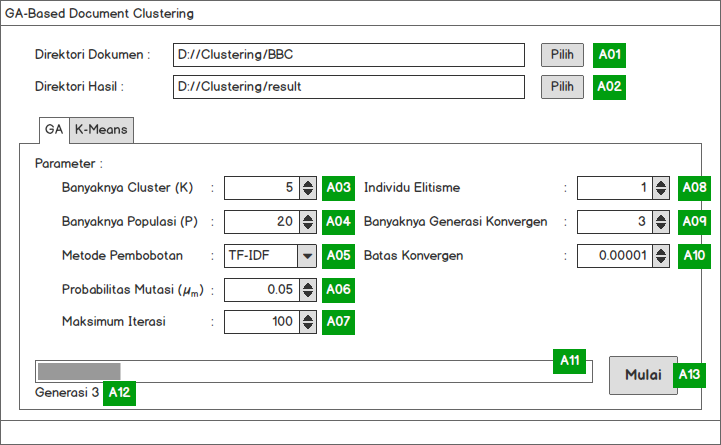
\includegraphics[width=0.7\textwidth]{UI/GA-Mockup}
		\caption{Rancangan antarmuka halaman algoritma genetika}
		\label{fig:UI-GA}
	\end{center}
\end{figure}

Penjelasan setiap \textit{field} dalam halaman ini dijelaskan dalam Tabel \ref{tbl:field-GA}.

\begin{table}[H]
	\renewcommand{\arraystretch}{2}
	\begin{tabularx}{\textwidth}{l X l X l X} \hline
		\textbf{Kode} & \textbf{Nama} & \textbf{Jenis} & \textbf{\textit{Defaut value}} & \textbf{Wajib} & \textbf{Aturan validasi} \\ \hline
		A01 & Direktori Dokumen & \textit{file chooser} & - & ya & - \\ \hline
		A02 & Direktori Hasil & \textit{file chooser} & - & ya & - \\ \hline
		A03 & Banyaknya Cluster & \textit{spinner} & 5 & ya & Nilai minimum 1 \\ \hline
		A04 & Banyaknya Populasi & \textit{spinner} & 1 & ya & Nilai minimum 1 dan harus lebih besar dari Individu Elitisme (A08) \\ \hline
		A05 & Metode Pembobotan & \textit{dropdown} & TF-IDF & ya & - \\ \hline
		A06 & Probabilitas Mutasi & \textit{spinner} & 0.05 & ya & Nilai minimum 0.01, maksimum 1.00 \\ \hline
		A07 & Maksimum Iterasi & \textit{spinner} & 100 & ya & Nilai minimum 1 dan harus lebih besar dari Banyaknya Generasi Konvergen (A09)\\ \hline
		A08 & Individu Elitisme & \textit{spinner} & 1 & ya & Nilai minimum 1 dan harus lebih kecil dari Banyaknya Populasi (A04)\\ \hline
		A09 & Banyaknya Generasi Konvergen & \textit{spinner} & 3 & ya & Nilai minimum 2 dan harus lebih kecil dari Maksimum Iterasi (A07) \\ \hline
		A10 & Batas Konvergen & \textit{spinner} & 0.00001 & ya & Hanya bisa bernilai $10^{-3}$, $10^{-4}$, $10^{-5}$, $10^{-6}$, dan $10^{-7}$ \\ \hline
	\end{tabularx}
	\caption{Rincian \textit{field} pada halaman algoritma genetika}
	\label{tbl:field-GA}
\end{table}

Objek dengan kode A11 merupakan sebuah \textit{progress bar} yang akan menampilkan perkembangan dari jalannya program untuk setiap iterasi. Apabila proses dalam suatu iterasi sudah selesai, maka akan mengubah nilai dari label A12 dan membuat \textit{progress bar} kembali kosong. Label dengan kode A12 berfungsi untuk menampilkan status dari program yang sedang berjalan. Label ini tidak akan memiliki nilai apabila program belum dijalankan dan akan menampilkan status "Inisialisasi..." apabila program sedang melakukan pengindeksan dokumen dan inisialisasi populasi. Setelah iterasi dimulai maka label A12 akan menampilkan generasi saat ini. Sebagai contoh apabila label A12 menampilkan status "Generasi 1" artinya saat ini program sedang melakukan proses-proses pada generasi 1. Begitu juga untuk "Generasi 2" dan seterusnya. Tombol dengan kode A13 berfungsi untuk memulai proses pengelompokan menggunakan algoritma genetika berdasarkan parameter yang telah dimasukkan.

\subsection{Halaman K-Means}

\begin{figure}[H]
	\begin{center}
		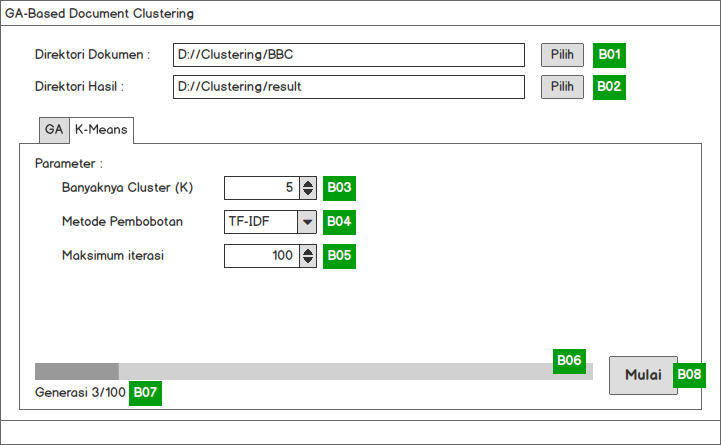
\includegraphics[width=0.7\textwidth]{UI/KMeans-mockup}
		\caption{Rancangan antarmuka halaman algoritma genetika}
		\label{fig:UI-KMeans}
	\end{center}
\end{figure}

Gambar \ref{fig:UI-KMeans} merupakan tampilan yang akan digunakan oleh pengguna untuk melakukan pengelompokan dokumen menggunakan algoritma K-Means. Berbeda dengan halaman algoritma genetika, pada halaman ini hanya terdapat tiga buah parameter yang dapat diubah-ubah oleh pengguna dalam melakukan pengelompokan.

\begin{table}[H]
	\renewcommand{\arraystretch}{2}
	\begin{tabularx}{\textwidth}{l X l X l X} \hline
		\textbf{Kode} & \textbf{Nama} & \textbf{Jenis} & \textbf{\textit{Defaut value}} & \textbf{Wajib} & \textbf{Aturan validasi} \\ \hline
		B01 & Direktori Dokumen & \textit{file chooser} & - & ya & - \\ \hline
		B02 & Direktori Hasil & \textit{file chooser} & - & ya & - \\ \hline
		B03 & Banyaknya Cluster & \textit{spinner} & 5 & ya & Nilai minimum 1 \\ \hline
		B04 & Metode Pembobotan & \textit{dropdown} & TF-IDF & ya & - \\ \hline
		B05 & Maksimum Iterasi & \textit{spinner} & 100 & ya & Nilai minimum 1\\ \hline
	\end{tabularx}
	\caption{Rincian \textit{field} pada halaman algoritma genetika}
	\label{tbl:field-GA}
\end{table}

Objek dengan kode B06 merupakan sebuah \textit{progress bar} yang akan menampilkan perkembangan dari jalannya program yang menyatakan banyaknya iterasi yang sudah selesai dijalankan dibandingkan dengan maksimum iterasi. Label B07 akan berisi keterangan dari proses yang sedang berlangsung. Salah satu contoh isi dari label B07 adalah "Iterasi 2/100" yang berarti saat ini sedang dilakukan pemrosesan pada iterasi kedua dari 100 iterasi. Tombol dengan kode B08 berfungsi untuk memulai proses pengelompokan menggunakan algoritma K-Means berdasarkan parameter yang telah dimasukkan.
